\documentclass[11pt,preprint, authoryear]{elsarticle}

\usepackage{lmodern}
%%%% My spacing
\usepackage{setspace}
\setstretch{1.2}
\DeclareMathSizes{12}{14}{10}{10}

% Wrap around which gives all figures included the [H] command, or places it "here". This can be tedious to code in Rmarkdown.
\usepackage{float}
\let\origfigure\figure
\let\endorigfigure\endfigure
\renewenvironment{figure}[1][2] {
    \expandafter\origfigure\expandafter[H]
} {
    \endorigfigure
}

\let\origtable\table
\let\endorigtable\endtable
\renewenvironment{table}[1][2] {
    \expandafter\origtable\expandafter[H]
} {
    \endorigtable
}


\usepackage{ifxetex,ifluatex}
\usepackage{fixltx2e} % provides \textsubscript
\ifnum 0\ifxetex 1\fi\ifluatex 1\fi=0 % if pdftex
  \usepackage[T1]{fontenc}
  \usepackage[utf8]{inputenc}
\else % if luatex or xelatex
  \ifxetex
    \usepackage{mathspec}
    \usepackage{xltxtra,xunicode}
  \else
    \usepackage{fontspec}
  \fi
  \defaultfontfeatures{Mapping=tex-text,Scale=MatchLowercase}
  \newcommand{\euro}{€}
\fi

\usepackage{amssymb, amsmath, amsthm, amsfonts}

\def\bibsection{\section*{References}} %%% Make "References" appear before bibliography


\usepackage[round]{natbib}

\usepackage{longtable}
\usepackage[margin=2.3cm,bottom=2cm,top=2.5cm, includefoot]{geometry}
\usepackage{fancyhdr}
\usepackage[bottom, hang, flushmargin]{footmisc}
\usepackage{graphicx}
\numberwithin{equation}{section}
\numberwithin{figure}{section}
\numberwithin{table}{section}
\setlength{\parindent}{0cm}
\setlength{\parskip}{1.3ex plus 0.5ex minus 0.3ex}
\usepackage{textcomp}
\renewcommand{\headrulewidth}{0pt}

\usepackage{array}
\newcolumntype{x}[1]{>{\centering\arraybackslash\hspace{0pt}}p{#1}}

%%%%  Remove the "preprint submitted to" part. Don't worry about this either, it just looks better without it:

 \def\tightlist{} % This allows for subbullets!

\usepackage{hyperref}
\hypersetup{breaklinks=true,
            bookmarks=true,
            colorlinks=true,
            citecolor=blue,
            urlcolor=blue,
            linkcolor=blue,
            pdfborder={0 0 0}}


% The following packages allow huxtable to work:
\usepackage{siunitx}
\usepackage{multirow}
\usepackage{hhline}
\usepackage{calc}
\usepackage{tabularx}
\usepackage{booktabs}
\usepackage{caption}


\newenvironment{columns}[1][]{}{}

\newenvironment{column}[1]{\begin{minipage}{#1}\ignorespaces}{%
\end{minipage}
\ifhmode\unskip\fi
\aftergroup\useignorespacesandallpars}

\def\useignorespacesandallpars#1\ignorespaces\fi{%
#1\fi\ignorespacesandallpars}

\makeatletter
\def\ignorespacesandallpars{%
  \@ifnextchar\par
    {\expandafter\ignorespacesandallpars\@gobble}%
    {}%
}
\makeatother

\newlength{\cslhangindent}
\setlength{\cslhangindent}{1.5em}
\newenvironment{CSLReferences}%
  {\setlength{\parindent}{0pt}%
  \everypar{\setlength{\hangindent}{\cslhangindent}}\ignorespaces}%
  {\par}


\urlstyle{same}  % don't use monospace font for urls
\setlength{\parindent}{0pt}
\setlength{\parskip}{6pt plus 2pt minus 1pt}
\setlength{\emergencystretch}{3em}  % prevent overfull lines
\setcounter{secnumdepth}{5}

%%% Use protect on footnotes to avoid problems with footnotes in titles
\let\rmarkdownfootnote\footnote%
\def\footnote{\protect\rmarkdownfootnote}
\IfFileExists{upquote.sty}{\usepackage{upquote}}{}

%%% Include extra packages specified by user

%%% Hard setting column skips for reports - this ensures greater consistency and control over the length settings in the document.
%% page layout
%% paragraphs
\setlength{\baselineskip}{12pt plus 0pt minus 0pt}
\setlength{\parskip}{12pt plus 0pt minus 0pt}
\setlength{\parindent}{0pt plus 0pt minus 0pt}
%% floats
\setlength{\floatsep}{12pt plus 0 pt minus 0pt}
\setlength{\textfloatsep}{20pt plus 0pt minus 0pt}
\setlength{\intextsep}{14pt plus 0pt minus 0pt}
\setlength{\dbltextfloatsep}{20pt plus 0pt minus 0pt}
\setlength{\dblfloatsep}{14pt plus 0pt minus 0pt}
%% maths
\setlength{\abovedisplayskip}{12pt plus 0pt minus 0pt}
\setlength{\belowdisplayskip}{12pt plus 0pt minus 0pt}
%% lists
\setlength{\topsep}{10pt plus 0pt minus 0pt}
\setlength{\partopsep}{3pt plus 0pt minus 0pt}
\setlength{\itemsep}{5pt plus 0pt minus 0pt}
\setlength{\labelsep}{8mm plus 0mm minus 0mm}
\setlength{\parsep}{\the\parskip}
\setlength{\listparindent}{\the\parindent}
%% verbatim
\setlength{\fboxsep}{5pt plus 0pt minus 0pt}



\begin{document}



\begin{frontmatter}  %

\title{The Church as a Lending Institution in the Cape Colony 1670 -
1710}

% Set to FALSE if wanting to remove title (for submission)




\author[Add1]{Harriet Catherine Laing}
\ead{21617023@sun.ac.za}





\address[Add1]{Stellenbosch University, Stellenbosch, South Africa}


\begin{abstract}
\small{
Abstract to be written here. The abstract should not be too long and
should provide the reader with a good understanding what you are writing
about. Academic papers are not like novels where you keep the reader in
suspense. To be effective in getting others to read your paper, be as
open and concise about your findings here as possible. Ideally, upon
reading your abstract, the reader should feel he / she must read your
paper in entirety.
}
\end{abstract}

\vspace{1cm}





\vspace{0.5cm}

\end{frontmatter}



%________________________
% Header and Footers
%%%%%%%%%%%%%%%%%%%%%%%%%%%%%%%%%
\pagestyle{fancy}
\chead{}
\rhead{}
\lfoot{}
\rfoot{\footnotesize Page \thepage}
\lhead{}
%\rfoot{\footnotesize Page \thepage } % "e.g. Page 2"
\cfoot{}

%\setlength\headheight{30pt}
%%%%%%%%%%%%%%%%%%%%%%%%%%%%%%%%%
%________________________

\headsep 35pt % So that header does not go over title




\hypertarget{introduction}{%
\section{\texorpdfstring{Introduction
\label{Introduction}}{Introduction }}\label{introduction}}

\hypertarget{background}{%
\section{\texorpdfstring{Background
\label{Literature}}{Background }}\label{background}}

The Cape Colony was first established in 1652 by Jan van Riebeeck and
was colonised to serve as a refreshment station for Vereenigde
Oostindische Compagnie (VOC) ships. The VOC was a company that was
chartered by the Dutch Republic's State General to act on behalf of its
colonized territories overseas (Fourie et al.~2012:51) and Van Riebeeck
was the Commander of the VOC at this time. The Cape was colonised to
address the high incidence of scurvy that the VOC sailors were prone to
falling sick to while on long ship voyages between Holland and the East
Indies (Fourie et al.~2012:55). The first settler population that
inhabited the Cape consisted of approximately two hundred individuals. A
large proportion of these first settlers were male, whereas women and
children constituted only five percent of the settlers' population
recorded in 1658 (Horner \& Wilson, 2008:8). In the same year, slaves
constituted 52 percent of the population; approximately half of which
were owned by the VOC and the other half owned by freemen (Horner \&
Wilson, 2008:8). By 1701, the population had grown to approximately 4
500 (at least based on those involved in the Cape economy) as more
European immigrants and slaves arrived in the Cape (Fourie \& van
Luiten, 2012).

Society in the Cape Colony consisted of four main groups, namely (i) the
settler population, (ii) the officials and personnel of the VOC, (iii)
the Khoesan (the original inhabitants of the Cape) and (iv) slaves. The
settler population consisted primarily of Dutch and German people from a
variety of socio-economic backgrounds; some were affluent or ``middle
class'' with debt burdens, and others poor and without land (Guelke,
1988:458). There was a further group included in the settler population
that originated from France. These immigrants were known as Huguenots
and had fled France because of the increased persecution of Protestants
in their origin country (Horner \& Wilson, 2008:14).

In the 1680s, many Huguenots were offered a free passage to the Cape and
advances for equipment that they would upon arrival by the VOC. These
inducements were provided upon the condition that the Huguenots pledged
an oath of allegiance to the VOC and remain there for at least five
years (Horner \& Wilson, 2008:14). The Huguenots were regarded by the
VOC as a potential asset to the Cape Colony, which is why they offered
inducements to this group to emigrate to the Cape (Wirgman, 1895:36).
However, the Commander of the VOC at this time did not regard the
Huguenot's assisted emigration favourably, because his policy approach
was to align the Cape Colony more closely with the Netherlands (Wirgman,
1895:36). Perhaps there was initial favoritism towards the Huguenots,
that later soured into discrimination following the change in
leadership's sentiment.

Slaves first arrived at the Cape in a small group in the year following
1652. In 1654, the first slaving expedition by the VOC from the Cape
obtained more slaves to bring back from Madagascar (Horner \& Wilson,
2008:5). Slaves were rarely allowed to become manumitted. However,
slaves could have their freedom purchased if a free man wished to marry
them. For example, a notable marriage through which one female slave was
manumitted was between a woman called Eva and a free man called Pieter
van Meerhof (Horner \& Wilson, 2008:9). It is likely that she is the
recorded ``Eva de Hottentotin'' in the data set, as it is recorded that
van Meerhof predeceased Eva before 1674. Therefore, the dates align and
women tended to receive loans from the church on behalf of their late
husbands.

It is well-documented that the VOC provided land and loans to settlers
that arrived in the Cape. For example, in 1657, the directors of the VOC
mandated that nine married, settler couples from Dutch and German origin
be given farmlands in an attempt to provide a steady supply of meat,
grain and wine, following unsuccessful efforts in this regard by VOC
slaves (Horner \& Wilson, 2008:7). Generally, these first farmers in the
Cape Colony were previously servants for the VOC that were manumitted.
As they were previously servants, they had little resources or capital
to use in their new farming ventures. Accordingly, the VOC provided some
tools and cattle, however, any investments that were required in excess
of these items had to come from the farmers themselves (Fourie \& Von
Fintel, 2009:8).

It is less clear what the role of the church as a lending institution in
the early Cape Colony was. It has been recorded that the church played a
role in giving money to farmers in need (Fourie \& Von Fintel, 2009:8).
In 1665, the first formal religious institution for the Dutch Reformed
Consistory was established at the Cape (Wirgman, 1895:23). The Dutch
Reformed Church in Cape Town was completed in 1703 (Wirgman, 1895:31).
The church addressed matters not only religious but also related to the
control of government. The importance of the church was great, as the
deacons of the Dutch Reformed church helped destitute individuals and
orphans (Wirgman, 1895:29). It is uncertain how much wealth the church
had throughout the period of interest, but in 1679 it was recorded that
the church had a capital fund of 1535 British pounds available for
charitable needs (Wirgman, 1895:29). However, the literature on the role
of church as an economic institution in the Cape is scarce.

\hypertarget{data}{%
\section{\texorpdfstring{Data \label{Data}}{Data }}\label{data}}

The data set used for this research were the 17 loan books of the church
in the Cape Colony spanning from 1670 to 1710, with some years missing.
Each loan book detailed the name of the loan recipient, the amount of
the loan, any interest accrued and a brief description thereof. This
data set includes a lot of persistent entries, as there are many
recurring loan recipients and loans amounts. In other words, it appears
that the same people in the Cape Colony receive loans from the church
year after year. However, what is less clear is whether these recurring
loan recipients are receiving a similar amount from the church each
year, or whether in some instances the initial amount lent is simply
repaid the following year, or is accruing interest.

As can be seen in Figure 1, there was a general upward trend in the
total amount of loans provided by the church from 1670 until 1710. The
year 1687 was omitted from this graph as it was an unusually sparse and
short loan book, compared to the rest of the years in the data set, and
distorted the average change over time. Similarly, the year 1687 was
dropped from the number of loan recipients in Figure 2. From Figure 1,
it is evidenced that the church provided more loans over time. However,
as discussed in section 2, the population of the Cape Colony increased
over this time period. Therefore, this graph is insufficient to
implicate that the influence of the loans granted by the church
increased. Albeit, it is still illustrated that the church increased it
lending capacity and had the ability to provide more capital to those
living in the Cape Colony in 1710 compared to 1670, an increase in
excess of 70 000 gulden.

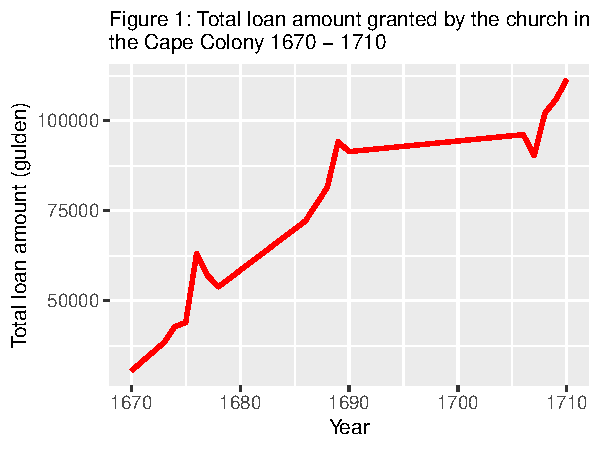
\includegraphics{HistoryEssay_files/figure-latex/unnamed-chunk-1-1.pdf}

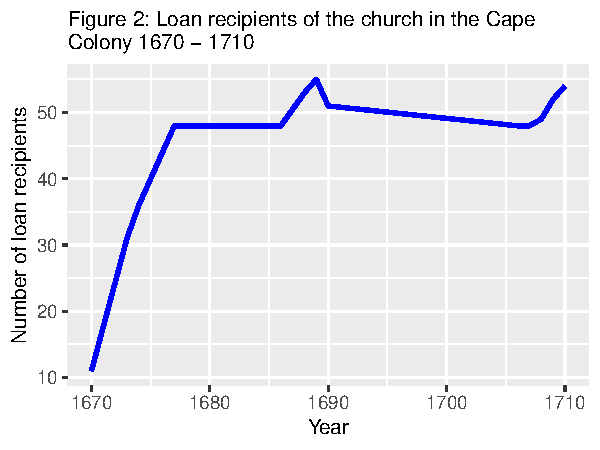
\includegraphics{HistoryEssay_files/figure-latex/unnamed-chunk-2-1.pdf}
For the number of loan recipients, there is less of a steady increase
over time. Figure 2 that depicts the number of individual loan
recipients in this period increased substantially from 1670 until 1678.
It is evident that after 1678, the number of individual loan recipients
stagnated and approximately 48 recipients received loans from the church
for the remainder of the period.

\hypertarget{methodology}{%
\section{\texorpdfstring{Methodology
\label{Meth}}{Methodology }}\label{methodology}}

The main research question was to investigate whether there was an
impact of the type of loan recipient on the loan amount granted by the
church. As aforementioned, the persistent nature of the data set needed
to be addressed. Accordingly, the initial observation for each loan
recipient was only included in the analysis of this paper. This resulted
in 145 observations. By using this isolation of only initial
observations, we attempt to control for the potential multi-collinearity
within the data set. Moreover, we created a dummy for each year included
in the data set. This was necessary because of the general upward trend
in the total amount of loans granted by the church over the time period.
Two years were dropped from the data set because they did not include an
initial observation.

To attempt to understand the effect of the type of loan recipient on the
loan amount granted by the church, it was necessary to create dummy
variables for the type of loan recipient. The first type identified in
the data set were those with surnames that indicated slave origin, which
amounted to 4 individuals. For example, those with surnames such as `van
Guinea' or `van Bengalen' indicated that these individuals originated
from countries from which slaves were obtained from. It is assumed that
these individuals with slave-origin surnames were manumitted in the Cape
Colony. The second type identified was women. It was rare to find women,
in fact only 7 women were recorded in the data set. It was clear from a
preliminary review of the data that slaves and woman received
significantly less loans than Huguenots or those in the Other category
type. The third type identified was the Huguenots. Using a list of
Huguenot family surnames (Fourie \& von Vintel, xx), these loan
recipients were categorised and amounted to 12 individuals. The
reference group for all individuals that did not fall into one of these
three aforementioned categories were listed as Other and constituted 128
individuals. However, to investigate whether these types had an effect
on the amount of the loan given by the church was determined using an
ordinary least squared regression, as follows:

\[
LoanAmount = x_0 + Huguenot \beta_1 + SlaveOrigin \beta_2 + Woman \beta_3 + YearDummy \beta_i + \varepsilon
\] where the dummy for year is a vector includes all the years that
contain initial observations for individual loan recipients, as a
coefficient to beta which is indexed by \(i=4, 5, 6...\).

Three regressions were run. First regression, all dummies for types and
years were included to determine the effect on loan amount. The
R-squared was found to be 0.218 and only the coefficients on the dummies
for years 1673, 1675 and 1710. Second regression, only the year dummies.
Dropped the insignificant type variables. Third regression, again
included all the dummies for both years and types and then included some
interaction terms too, however, still could not find type to be
significant in finding an effect of loan recipient type on loan amount.

\hypertarget{limitations}{%
\section{\texorpdfstring{Limitations
\label{Limitations}}{Limitations }}\label{limitations}}

Omitted variable bias

Small sample: only 145 observations, of which

As aforementioned, there are many years missing in the church loan
books. It can be assumed that year on year, an omission of a singular
year may not bias our results on average. However, a concern arises
regarding the longer time periods for which there is no record of loans.
For example, in this particular data set there are two large gaps: from
1678 to 1686 and from 1690 to 1706. The reason for concern in the case
of the methodology applied in this research is that the observations
included were those of the first loan recorded to a loan recipient.
Accordingly, it is likely that after a long period of missing years, the
following available year will be upward biased in terms of its impact on
the loan amount. This can be seen in the fact that 1706 was the
reference group for the year dummy.

\hypertarget{discussion}{%
\section{\texorpdfstring{Discussion
\label{Discussion}}{Discussion }}\label{discussion}}

In addition to revenue generated from trading and commercial activites
in addition to taxes levied on settlers in the Cape Colony (Fourie et
al.~2012: 59-62), the VOC received loans from the church. However, as
calculated by Fourie et al.~(2012) the VOC generated approximately 50
000 gulden in the years of 1700 and 1705, so the amounts recorded in the
church loan books may not have contributed much. For four years from
1670, the church loaned 992 gulden to the VOC and then in 1706, it
loaned 4000 gulden.

Further research, likelihood of receiving loans again year on year for
the periods in the data set without significant gaps. Perhaps there was
not discrimination in the amount of the loans given, but perhaps levied
more interest on freed slaves than for free burghers.

\hypertarget{conclusion}{%
\section{\texorpdfstring{Conclusion
\label{Conclusion}}{Conclusion }}\label{conclusion}}

\newpage

\hypertarget{references}{%
\section*{References}\label{references}}
\addcontentsline{toc}{section}{References}

Guelke, L. 1988. The Anatomy of a Colonial Settler Population: Cape
Colony 1657-1750. \_The International Journal of African Historical
Studies, 21(3):453-473.

Fourie, J., Jansen,A. \& Siebrits, K. 2012. Public finances under
private company rule: The Dutch Cape Colony (1652-1795).

Horner, D. \& Wilson, F. 2008. A Tapestry of People: The Growth of
Population in the Province of the Western Cape. A Southern Africa Labour
and Development Research Unit Working Paper No 21. Cape Town: SALDRU,
University of Cape Town.

Fourie, J., Jansen,A. \& Siebrits, K. 2012. Public finances under
private company rule: The Dutch Cape Colony (1652-1795).

Fourie, J. \& Von Fintel, D. 2009. The dynamics of inequality in a newly
settled, pre-industrial society: The case of the Cape Colony.
Stellenbosch Economic Working Papers 17. Stellenbosch University.

J Fourie, ``The remarkable wealth of the Dutch Cape Colony: Measurements
from eighteenth-century probate inventories'', The Economic History
Review. 66(2), 2013, pp.~419--448.

?book Wirgman, A. T. 1895. The History of the Church in South Africa.
p13-49.
\url{https://repository.up.ac.za/bitstream/handle/2263/12783/002_p13-49.pdf?sequence=6\&isAllowed=y}.

\hypertarget{refs}{}
\begin{CSLReferences}{0}{0}
\end{CSLReferences}

\hypertarget{appendix}{%
\section*{Appendix}\label{appendix}}
\addcontentsline{toc}{section}{Appendix}

\begin{figure}
\centering
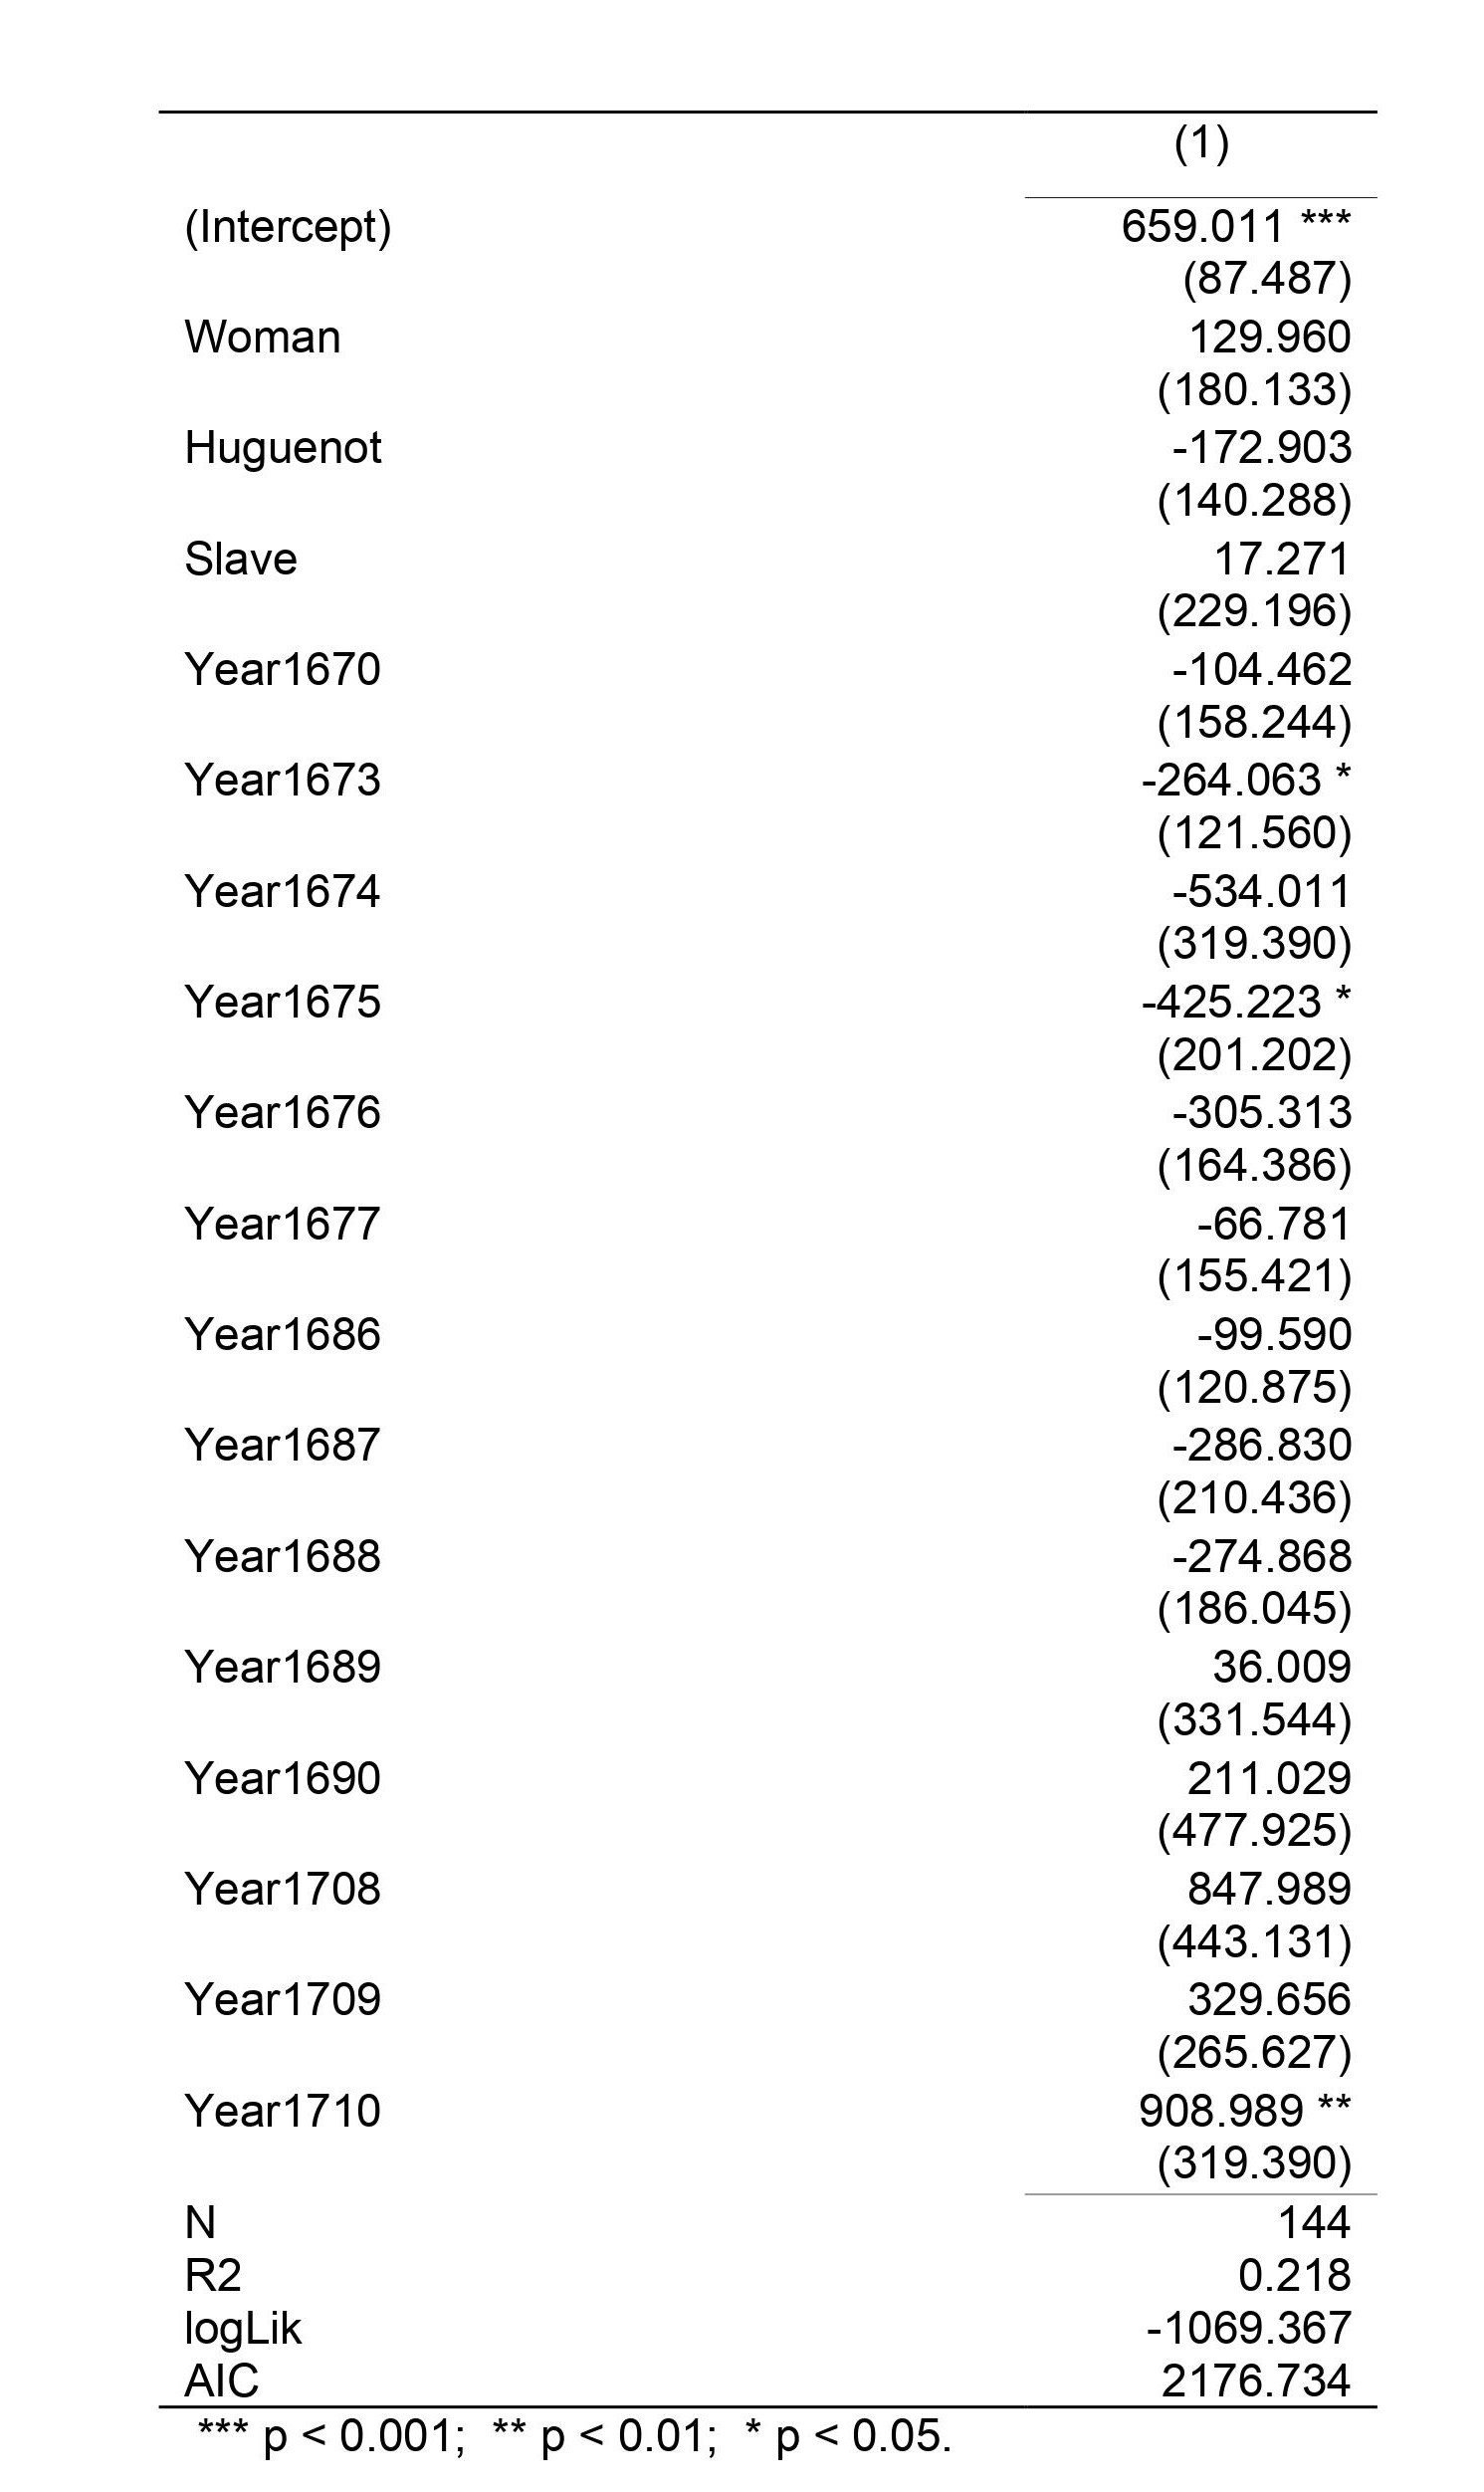
\includegraphics{/Users/Harriet/Documents/Economic History/ESSAY/Texevier_History_Essay/HistoryEssay/data/Reg1.jpg}
\caption{Alt Text}
\end{figure}

\bibliography{Tex/ref}





\end{document}
